\section{Introduction}
\label{sec:introduction}

Cyber-physical systems (CPS) are next generations of networked and
embedded systems, tightly coupled with computation and physical
elements to control real-world phenomenon.
Control algorithms of CPS, therefore, are becoming more and more
complex, which makes CPS distinguished from traditional safety-critical
systems.
In CPS applications, ``real-fast'' is often as important as ``real-time'',
while safety-critical systems are likely to have only the real-time
constraint. 
Such a double-edge real-time and real-fast requirement of CPS, however,
has imposed a core challenge on systems technology.
In this paper, we tackle this problem with a specific example of plasma
control.

Plasma control for fusion is an applications of energy CPS, where
complex algorithms must be computed at a very high rate.
Figure~\ref{fig:tokamak} shows the HBT-EP Tokamak at Columbia
University~\cite{Maurer_PPCF11,Rath_FED12} that magnetically controls
the 3-D perturbed equilibrium state of the plasma~\cite{Boozer_PP99}.
It is required to process 96 inputs and 64 outputs of 16-bit data at a
sampling rate of a few microseconds.
An initial attempt of the Columbia team employed fast CPUs or FPGAs, but
even the simplified algorithm failed to run within 20$\mu$s.
An alternative approach was to parallelize the algorithm using the
graphics processing unit (GPU) and CUDA~\cite{CUDA} -- the most
successful massively parallel computing technology.
However, the current system for GPU computing is not designed to
integrate sensor and actuator devices with the GPU.
This is attributed to the fact that the current software stack
of GPU computing is independent of I/O device drivers.
Since it might take tens of microseconds to transfer hundreds-of-bytes
data between the CPU and the GPU, it is not affordable for the current
software stack to apply the GPU for plasma control in real-time.
This is a signficant problem not only for plasma control but also for
any applications of CPS that are augmented with compute devices.

\begin{figure}[t]
 \centering
 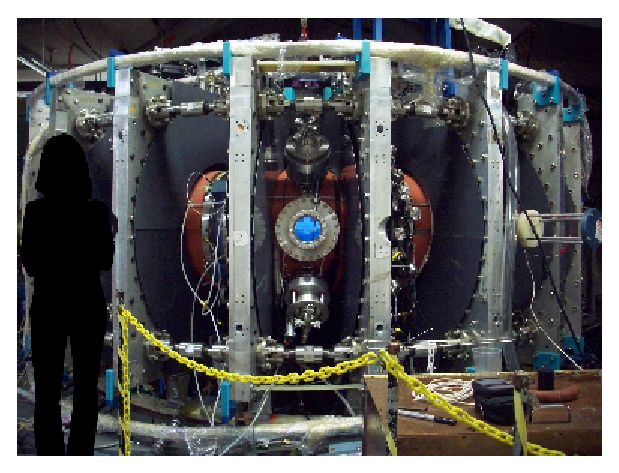
\includegraphics[width=0.78\hsize]{eps/tokamak.eps}
 \caption{The HBT-EP ``Tokamak'' at Columbia University.}
 \label{fig:tokamak}
\end{figure}

In order to utilize the GPU for applications of CPS, the system is
required to support a method of bypassing data transfer between the CPU
and the GPU, instead connecting the GPU and I/O devices directly.
To the best of our knowledge, however, there is currently no generic
systems support for such a direct data transfer machanism except for
specialized commercial products for the InfiniBand
network~\cite{GPUDirect}.
As a way of eliminating the data transfer cost between the CPU and the
GPU, the current programming framework often supports host memory
allocation, which enables the GPU to access data on the host memory;
however, it is unclear if this scheme is best suited for low-latency GPU
computing, because the data access to the host memory from the GPU is
expensive.
Given that GPUs are increasingly deployed in the domain of
CPS~\cite{Hirabayashi_REACTION12, Mangharam11, McNaughton_ICRA11,
Michel_IROS07}, 
and basic real-time resource management techniques for the GPU started to be
disclosed \cite{Elliott_RTS12, Elliott_ECRTS12, Kato_RTAS11,
Kato_RTSS11, Kato_ATC11, Kato_ATC12, Liu_PACT12}, it is time to look
into a tight integration of I/O processing and GPU computing.

\textbf{Contribution:}
In this paper, we present a zero-copy I/O processing scheme for GPU
computing.
This scheme enables I/O devices to directly transfer a limited size of
data to and from the GPU, by coordinating their device drivers. 
We also investigate a possibility of the exisiting schemes to support
low-latency GPU computing, and identify an advantage of our new scheme.
To do so, we provide a case study using the Columbia University's
Tokamak plasma control system that demonstrates an effect of our
new scheme on a sampling period of plasma control.
Furthermore, we provide microbenchmarking results to evaluate more
generic properties of the I/O processing schemes
By clarifying these capabilities, we aim to not only improve the overall
performance but also broaden the scope of CPS that can benefit from the
state-of-the-art GPU computing technology.

\textbf{Organization:}
The rest of this paper is organized as follows.
Section~\ref{sec:system_model} describes the system model and
assumptions behind this paper.
Section~\ref{sec:io_processing} proposes our zero-copy I/O processing
scheme, and differentiates it from the exisiting schemes.
Section~\ref{sec:implementation} presents details of system
implementation.
In Section~\ref{sec:case_study}, a case study of plasma control is
provided to demonstrate the real-world impact of our contribution.
Microbenchmarks are also used to evaluate more generic properties of the
I/O processing schemes in Section~\ref{sec:benchmarking}.
Section~\ref{sec:related_work} introduces related work, and this paper
concludes in Section~\ref{sec:conclusion}.